\documentclass{article}
\usepackage[utf8]{inputenc}

\newcommand\tens[1]{\underline{\underline{#1}}}
\newcommand\ve[1]{\underline{#1}}
\usepackage[utf8]{inputenc}     % for éô
\usepackage[a4paper, left=0.8in, right=0.8in, top=1in, bottom=1in]{geometry}
                                % for page size and margin settings
\usepackage{graphicx}           % for ?
\usepackage{float}
\usepackage{subfigure} 
\usepackage[squaren, Gray, cdot]{SIunits}
\usepackage{xspace}
\usepackage{array}
\usepackage{multirow}
\usepackage{amsmath,amssymb}    % for better equations
% \DeclareMathOperator{\commande}{texte}
\usepackage{amsthm}             % for better theorem styles
\usepackage{mathtools}          % for greek math symbol formatting
\usepackage{enumitem}           % for control of 'enumerate' numbering
\usepackage{listings}           % for control of 'itemize' spacing
\usepackage{todonotes}          % for clear TODO notes
\usepackage{newcent}            %pour la police
\usepackage{hyperref}           % page numbers and '\ref's become clickable
%%%%%%%%%%%%%%%%%%%%%%%
% \usepackage[usenames,dvipsnames]{color}
% \usepackage[numbered,framed]{mcode}
%%%%%%%%%%%%%%%%%%%%%%%
\newcommand\ul[1]{\underline{#1}}
\newcommand\uul[1]{\underline{\underline{#1}}}
\newcommand\uex{\ul{e}_x}
\newcommand\uey{\ul{e}_y}
\newcommand\uGrad{\ul{\nabla}}
%%%%%%%%%%%%%%%%%%%%%%%

\begin{document}
\lstset{language=matlab}   

\begin{titlepage}
	\thispagestyle{empty}
	\newcommand{\HRule}{\rule{\linewidth}{0.5mm}}
	\center
	\textsc{\large ECOLE NATIONALE DES PONTS ET CHAUSSEES}\\[.7cm]
	
\includegraphics[width=35mm]{img/ENPC_logo.png}\\[.5cm]
	\textsc{\large Departement Génie Mécanique et Matériaux - 2019/2020}\\[0.5cm]
	
	\vspace{2cm}
	
	\HRule \\[0.4cm]
	{\LARGE {\fontfamily{pag}\selectfont {SPH : Projet}}
    \vspace{0.4cm}
	\HRule \\[.5cm]

\vspace{3cm}

\large Réalisé par : 

\vspace{0.5cm}

{\fontfamily{pag}\selectfont{{\bfseries Andrey LATYSHEV} $\And$ {\bfseries Siyuan HE}}}
\\
\vspace{1cm}

% Encadré par : \bfseries\fontfamily{pag}\selectfont{Daniel Weisz-Patrault}

}
\end{titlepage}

% \newpage
% \vspace*{\stretch{1}}
% \begin{center}
%     \tableofcontents
% \end{center}
% \vspace*{\stretch{1}}

\newpage
\section{Implémentation d'un schéma de diffusion de densité}
Modèle de Molteni et Colagrossi: 
\begin{align*}
	\dot{\rho}_a &= -\rho_{a}D_{a}\{\ul{v}_{b}\}+\nu_{\rho}L_{a}\{\rho_{b}\}\\
	\nu_{\rho} &= \delta\sigma c_{0}, 
\end{align*}
où $\sigma=\sqrt{5/18}h$ si on prends noyau "Wendland $C^2$ ($d=2$)". $c_0$ est un constant déjà calculé. Ce que on doit ajouter dans le code est justement la terme laplacienne du $\rho$.

Car $\ul{\nabla}w_{ab} \propto \ul{r}_{ab}$ et $V_b = \frac{m}{\rho_b}$ on obtient
\begin{align*}
    L_{a}\{ \rho_{b} \} & = 2 \sum_b V_b(\rho_a - \rho_b)\frac{ \ul{r}_{ab} \cdot \uGrad w_{ab} }{ |\ul{r}_{ab}|^2 } = 2 \sum_b \frac{m}{\rho_b}(\rho_a - \rho_b)\frac{ |\uGrad w_{ab}| }{ |\ul{r}_{ab}| } \\
    D_{a}\{\ul{v}_{b}\} & = -\frac{1}{\rho_a} \sum_b m(\ul{v}_a - \ul{v}_b) \cdot \uGrad w_{ab} = -\frac{m}{\rho_a} \sum_b (\ul{v}_a - \ul{v}_b) \cdot \ul{r}_{ab} \frac{ | \uGrad w_{ab} | }{ |\ul{r}_{ab}| } \\
	-\rho_{a}D_{a}\{\ul{v}_{b}\}+\nu_{\rho}L_{a}\{\rho_{b}\} &= m\sum_b \left( (\ul{v}_a - \ul{v}_b) \cdot \ul{r}_{ab}  + 2 \nu_\rho \frac{\rho_a - \rho_b}{\rho_b} \right)  \frac{ |\uGrad w_{ab}| }{ |\ul{r}_{ab}| }
\end{align*}

On a pris TD2 comme une base de notre projet. Pour d'activer et de désactiver la diffusion de densité, On définit un variable "DENSDIFFTYPE" en égalant 1 ou 0 du ligne 83 à 86 (nommé par " Density diffusion (PROJECT!!!)"). Et le paramètre $\delta$ est laissé libre à utilisateur du ligne 88 (nommé par "diff Parameters").\par
  
\subsection{Impact sur le champs de pression}
On a implémenté le schéma de diffusion de densité de Molteni et Colagrossi dans la fonction \\
\lstinline$src\solver\DivergenceContribMolteniColagrossi.m$ :
\begin{lstlisting}           
function F = DivergenceContribMolteniColagrossi(m,dwdr,rVel,rPos,nu_rho,rho_i,rho_j)
rNorm = (rPos(:,1).*rPos(:,1)+rPos(:,2).*rPos(:,2)).^(.5);
veldotpos = rVel(:,1).*rPos(:,1)+rVel(:,2).*rPos(:,2);
F = m*veldotpos.*dwdr./rNorm + nu_rho*2*m*(rho_i-rho_j)./rho_j.*dwdr./rNorm;
end
\end{lstlisting} 

Pour appliquer ce schéma on a changé la détermination de la densité dans la fichier \\
\lstinline$src\solver\ComputeForces.m$ :

\begin{lstlisting}           
	%CONTINUITY CONTRIBUTION
	switch d
	case{2}
	sigma=sqrt(5/18)*h;
	nu_rho=delta*sigma*c0;
	case{3}
	sigma=sqrt(4/15)*h;
	nu_rho=delta*sigma*c0;
	end
	if DENSDIFFTYPE == COLAGROSSIDIFF
	dRhodt = 
	DivergenceContribMolteniColagrossi(m,dwdr,rVelCont,rPos,nu_rho,rho_i,rho_j);
	else
	dRhodt = DivergenceContrib(m,dwdr,rVelCont,rPos);
	end
\end{lstlisting} 

\begin{figure}[H]
	\begin{minipage}[H]{0.49\linewidth}
		\center{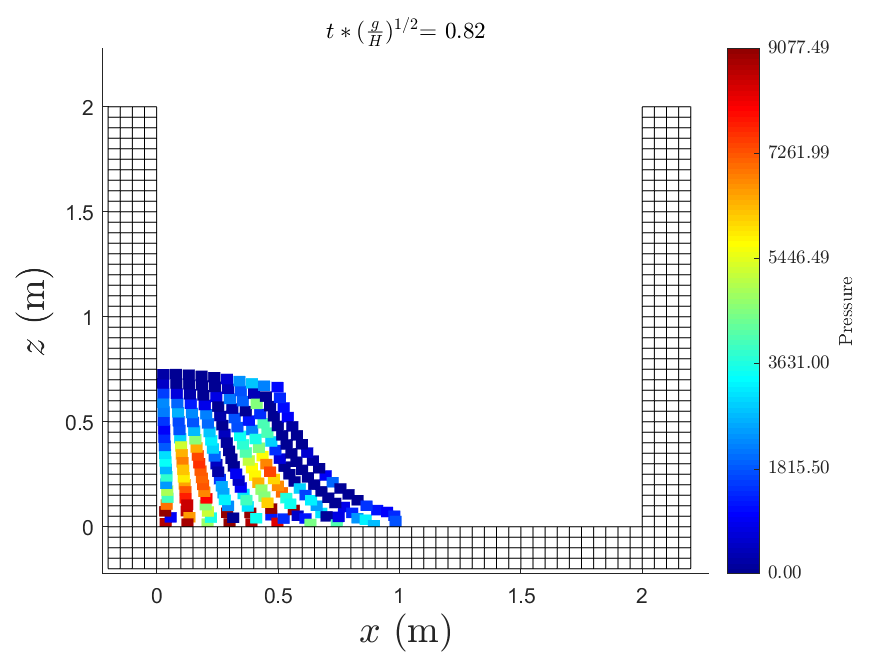
\includegraphics[width=1\linewidth]{img/alpha01delta00t082.png} }
		{$\alpha=0.1$ $\delta=0.0$}
	\end{minipage}
	\hfill
	\begin{minipage}[H]{0.49\linewidth}
		\center{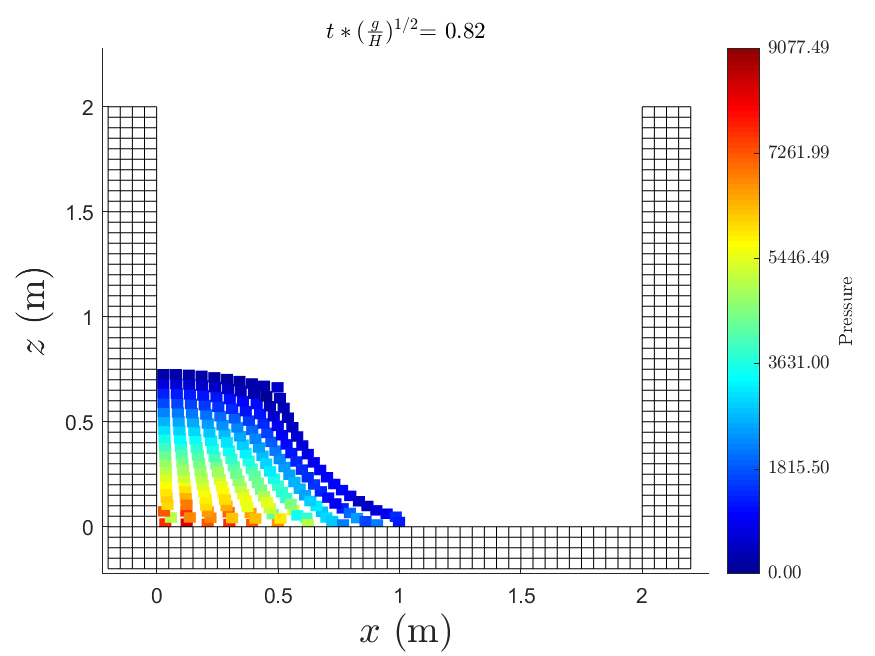
\includegraphics[width=1\linewidth]{img/alpha01delta02t082.png} }
		{$\alpha=0.1$ $\delta=0.2$}
	\end{minipage}
	\caption{Champ de pression comparé à un instant avec et sans diffusion de densité.}
\end{figure}
On voit facilement le champs de pression varie d'une manière "glissante" par rapport à gauche où on désactive la diffusion de densité. Ce schéma nous permets de simuler un processus dans lequel l'impact de la pression à la densité n'est pas négligeable. Celui-ci évite évidemment la divergence de l'itération dans calculs.

\subsection{Énergie mécanique en fonction du temps}
\begin{figure}[H]
	\begin{minipage}[H]{0.49\linewidth}
		\center{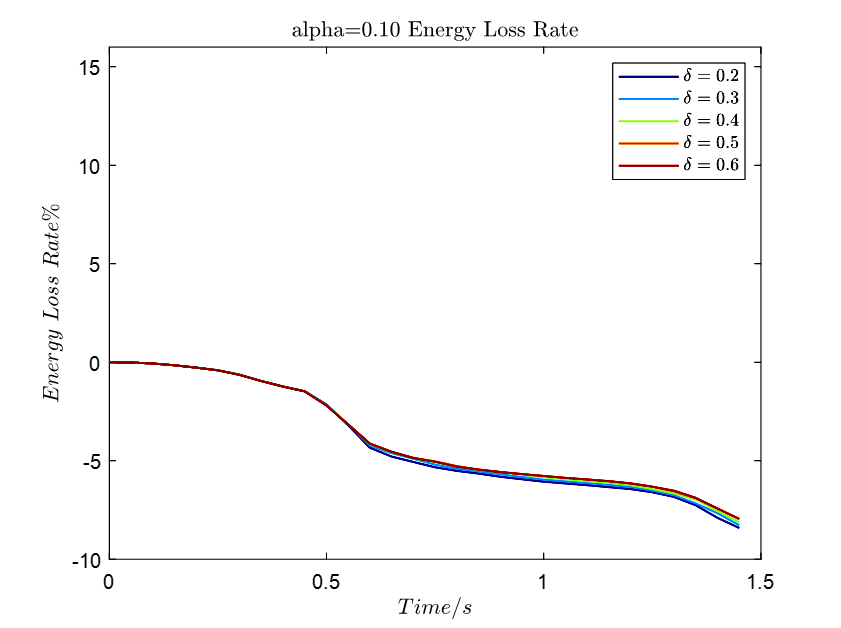
\includegraphics[width=1\linewidth]{img/em_al01.png} }
		{$\alpha=0.1$ $\delta$ varié}
	\end{minipage}
	\hfill
	\begin{minipage}[H]{0.49\linewidth}
		\center{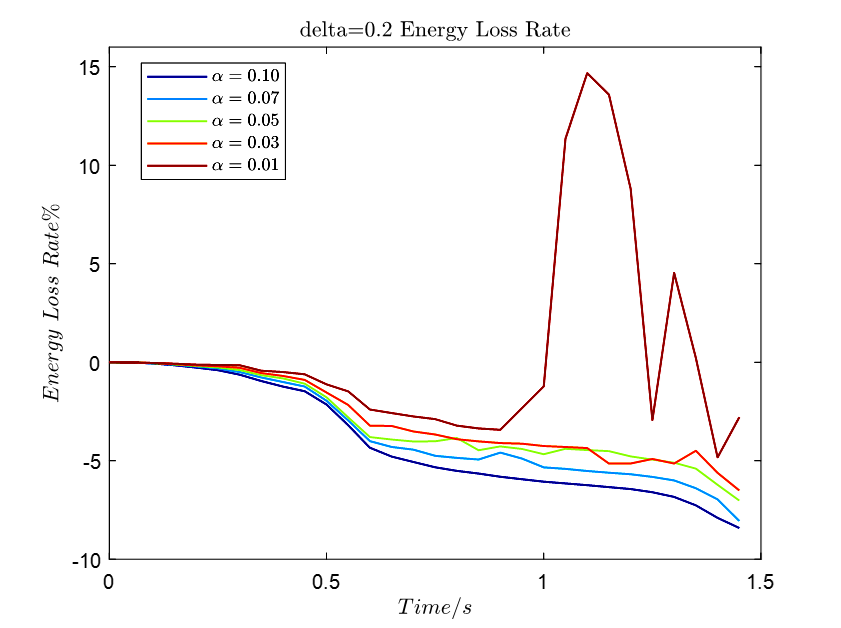
\includegraphics[width=1\linewidth]{img/em_de01.png} }
		{$\alpha$ varié $\delta=0.1$}
	\end{minipage}
	\caption{Énergie mécanique en fonction du temps}
\end{figure}

Dans cette partie-là, on ajoute une variable "$EnergyMeca$" dans le module "$INTEGRATION STEP$". Dans le module "$save the mecanic energy$",on enregistre l'énergie mécanique de cette système à certaine instant contrôlé par le variable "$t_em$" mis devant le début de l'itération. Pour mieux visualiser la variation de l'énergie mécanique, on calcule le taux de la perte d'énergie mécanique par rapport à l'état initial.

Premièrement la différence entre la courbe gauche et la courbe droite démontre le changement de $\delta$ ayant une perturbation faible sur la perte d'énergie. De l'image à droite, on vérifie d'abord que la limite inférieur de $\alpha$ égale $0.03$. Si on le diminue encore, l'itération va diverger ultérieurement. Cette conclusion coïncide avec l'énoncé du projet.

Et puis, on remarque que l'augmentation de $\delta$ conduit à une perte plus petite, au contraire l'augmentation de $\alpha$ conduit à une perte plus grande. Cette phénomène nous inspire que la viscosité artificielle rend l'itération robuste avec un coût de la perte d'énergie. Mais la diffusion de densité ne change pas beaucoup l'énergie mécanique totale. 
          
\subsection{Pression interpolée à la position x=2m et z=0.2m}
Pour trace la pression d'un certain point, il faut trouver le nombre de ce point. On utilise la fonction "find" pour fournir la critère "x==2m" et "z==0.2m". 
\begin{lstlisting}
	[observe_point,~]=find(abs(part(:,POS(1))-2.0)<=dr/2);%x==2.0m
	[observe_point_0,~]=find(abs(part(observe_point,POS(2))-0.2)<=dr/2);%z==0.2m
	observe_point=observe_point(observe_point_0);
\end{lstlisting}
la phrase "abs(part(:,POS(1))-2.0)<=dr/2" nous permet de trouver le point qui se trouve plus proche de (2,0.2). "dr" est le rayon du noyau. Une fois on le trouve, on peut chercher la pression interpolé en utilisant la variable "part". 
\begin{figure}[H]
	\begin{center}
		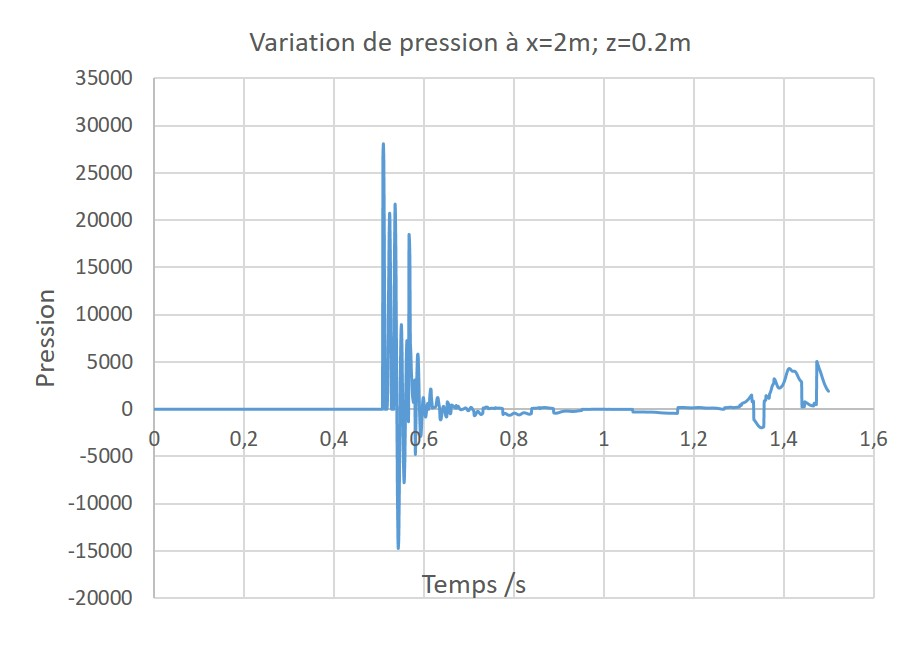
\includegraphics[width=10cm]{img/VariationPression.jpg}
	\end{center}
	\caption{Pression interpolée à la position x=2m et z=0.2m}
\end{figure}
   
On trace la pression d'un point $z=0.2m$, qui se trouve au mur à droite sur la base du barrage. Quand $t=0.5~0.6$, la pression oscille brutalement et on voit une perte d'énergie évidente dans la Figure 2. 
\begin{figure}[H]
	\begin{minipage}[H]{0.49\linewidth}
		\center{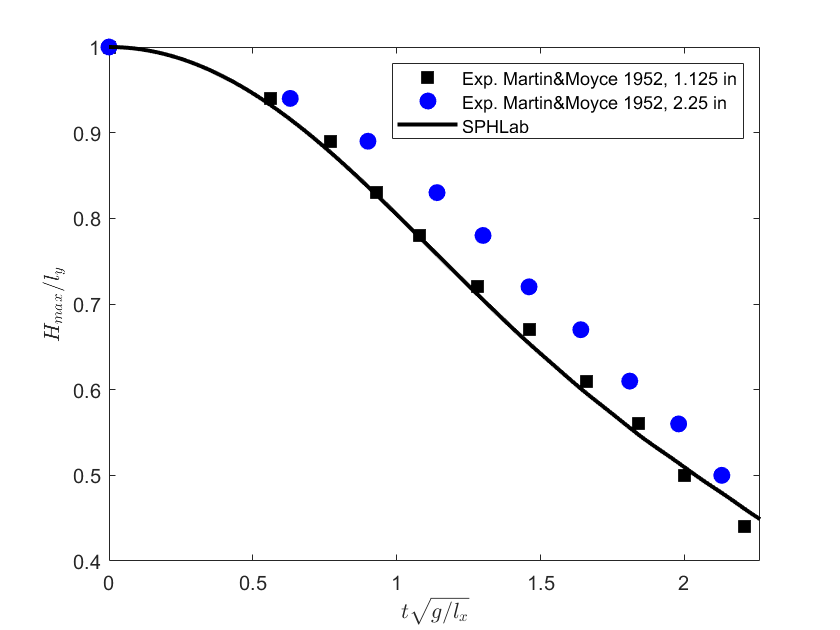
\includegraphics[width=1\linewidth]{img/numexpH_al01de02.png} }
		{$\alpha=0.1$ $\delta$ varié}
	\end{minipage}
	\hfill
	\begin{minipage}[H]{0.49\linewidth}
		\center{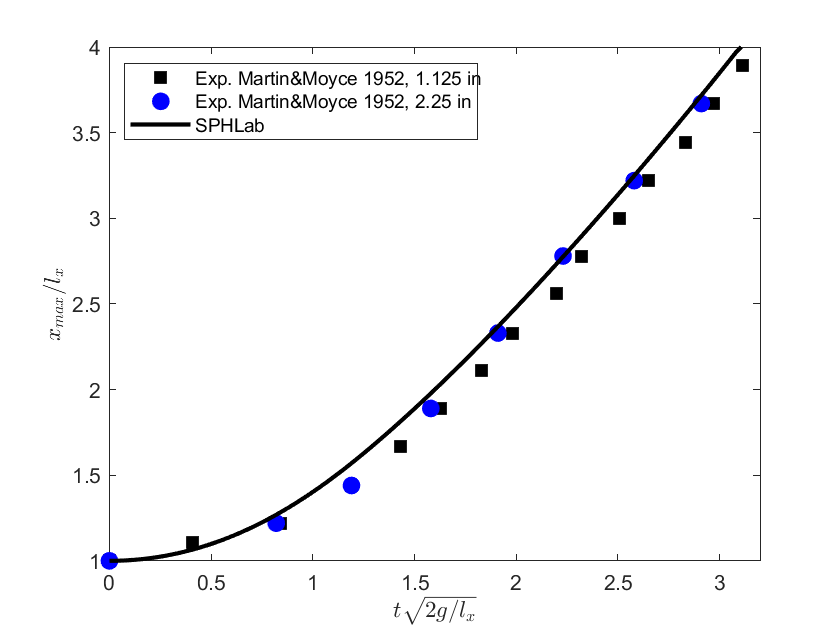
\includegraphics[width=1\linewidth]{img/numexpX_al01de02.png} }
		{$\alpha$ varié $\delta=0.1$}
	\end{minipage}
	\caption{Résultats expérimentaux et numériques}
\end{figure}

On compare nos résultats numériques avec les résultats expérimentaux donnés en séance TD2. On mets les paramètres $\alpha=0.1$ et $\delta=0.2$.\\ 
     
\section{Détection de surface libre}

Dans cette partie on va réaliser la méthode de détection de surface libre par Doring (2005). On a la matrice de renormalisation :
\begin{equation*}
	\uul{R}_i^{-1} = - \sum_{j} V_j \ul{\nabla} w_{ij} \otimes \ul{r}_{ij}
\end{equation*}
Car $\ul{\nabla}w_{ij} \propto \ul{r}_{ij}$ et $V_j = \frac{m}{\rho_j}$ on obtient
\begin{align*}
	& \uul{R}_i^{-1} = - \sum_{j} \frac{m}{\rho_j} \ul{\nabla} w_{ij} \otimes \ul{r}_{ij} = - m \sum_{j} 
	\frac{| \ul{\nabla} w_{ij} |}{\rho_j |\ul{r}_{ij} |} \ul{r}_{ij} \otimes \ul{r}_{ij} = -m A \implies A = A^T \\
	& A = \sum_j \frac{| \ul{\nabla} w_{ij} |}{\rho_j |\ul{r}_{ij} |} \left[ (r_{ij}^x)^2 \uex \otimes \uex + (r_{ij}^y)^2 \uey \otimes \uey + (r_{ij}^x r_{ij}^y)^2 (\uex \otimes \uey + \uey \otimes \uex) \right] \\ 
	& \lambda_{\min} = \min\lambda(\uul{R}_i^{-1}) = \min\{ -\frac{m}{2} (\mathrm{tr} A \pm \sqrt{\mathrm{tr}^2 - 4 \det A}) \} = -\frac{m}{2} (\mathrm{tr} A + \sqrt{\mathrm{tr}^2 - 4 \det A})
\end{align*}

Pour réaliser cette fonctionnalité on a implémenté des variables de type des particules et la fonction \lstinline$src\solver\particle_type.m$, qui retourne une liste de deux éléments : la valeur propre minimale et le type de la particule considérée.
% \\ \lstinline$LONELY_PARTICLE FREE_BOUNDARY_PARTICLE SURROUNDED_PARTICLE$
\begin{lstlisting}           
function particle_type = findParticleType(m,dwdr,rho_j,rPos)
    % R-1 = -m * A 
    global LONELY_PARTICLE FREE_BOUNDARY_PARTICLE SURROUNDED_PARTICLE;

    rNorm = sqrt(rPos(:,1).*rPos(:,1)+rPos(:,2).*rPos(:,2)); 
    a11_ij = dwdr.*rPos(:,1).*rPos(:,1)./(rho_j.*rNorm); 
    a12_ij = dwdr.*rPos(:,1).*rPos(:,2)./(rho_j.*rNorm); 
    a22_ij = dwdr.*rPos(:,2).*rPos(:,2)./(rho_j.*rNorm); 
    a11 = sum (a11_ij);
    a12 = sum (a12_ij);
    a22 = sum (a22_ij);
    trA = a11 + a22;
    detA = a11 * a22 - a12 * a12;
    lambda = -m * 0.5 * (trA + sqrt(trA * trA - 4 * detA));

    if lambda <= 0.2 
        particle_type = [lambda LONELY_PARTICLE];
    elseif (lambda > 0.2) && (lambda <= 0.75 ) 
        particle_type = [lambda FREE_BOUNDARY_PARTICLE];
    else 
        particle_type = [lambda SURROUNDED_PARTICLE];
end
\end{lstlisting} 

Pour déterminer tous les types des particules on a réalisé une fonction \lstinline$src\solver\separateParticles.m$, où il y a une boucle pour les particules \lstinline$FLUID$ de notre domaine. Cette fonction retourne trois listes : \lstinline$lambda_list$ contient toutes les valeurs propres minimales $\lambda_{\min}$, \lstinline$free_boundary_particles$ contient les indexes des particules appartenant à la surface libre et  \lstinline$lonely_particles$ contient les indexes des particules, qui appartiennent à un jet ou sont isolées.

Pour appliquer la fonctionnalité réalisé dans le projet, on appel la fonction \lstinline$separateParticles$ dans le fichier principale \lstinline$main_Part4.m$ sur chaque itération du processus. 
\begin{lstlisting}           
    [lonely_particles free_boundary_particles lambda_list] 
    = separateParticles(part,space);
\end{lstlisting} 

Pour s'assurer que l'algorithme détermine correctement la surface libre, on a changé un peu la fonction \lstinline$plotParticlesPressure$. Désormais, les carrées rouges indiquent la surface libre.  

\begin{lstlisting}
    % PLOT FREE BOUNDARY
    N = size(free_boundary_particles);
    for i = 1:N(2)
        k = free_boundary_particles(1,i);
        xtab = [part(k,POS(1))-dr/2 part(k,POS(1))+dr/2 
            part(k,POS(1))+dr/2 part(k,POS(1))-dr/2]';
        ytab = [part(k,POS(2))-dr/2 part(k,POS(2))-dr/2 
            part(k,POS(2))+dr/2 part(k,POS(2))+dr/2]';
        patch(xtab,ytab,'red');
    end
\end{lstlisting} 


\begin{figure}[H]
    \begin{minipage}[h]{0.32\linewidth}
        \center{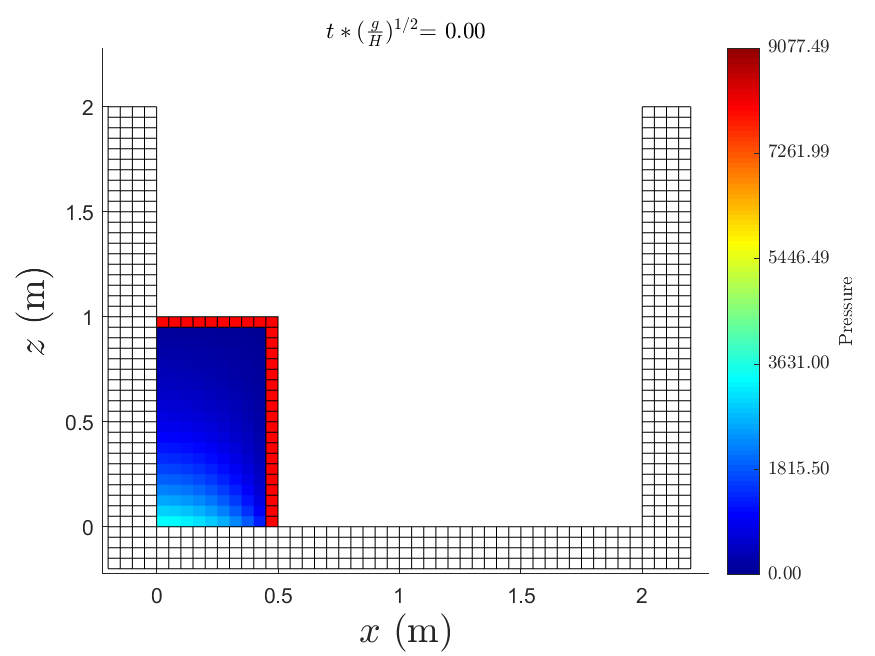
\includegraphics[width=1\linewidth]{img/sl/fig_000000}}
    \end{minipage}
    \hfill
    \begin{minipage}[h]{0.32\linewidth}
        \center{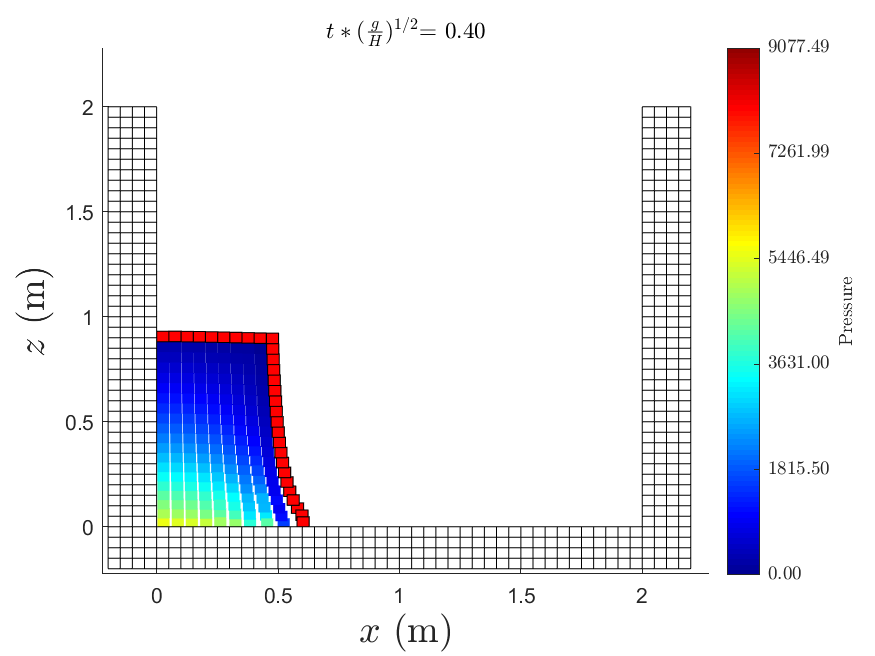
\includegraphics[width=1\linewidth]{img/sl/fig_000020}}
    \end{minipage}
    \hfill
    \begin{minipage}[h]{0.32\linewidth}
        \center{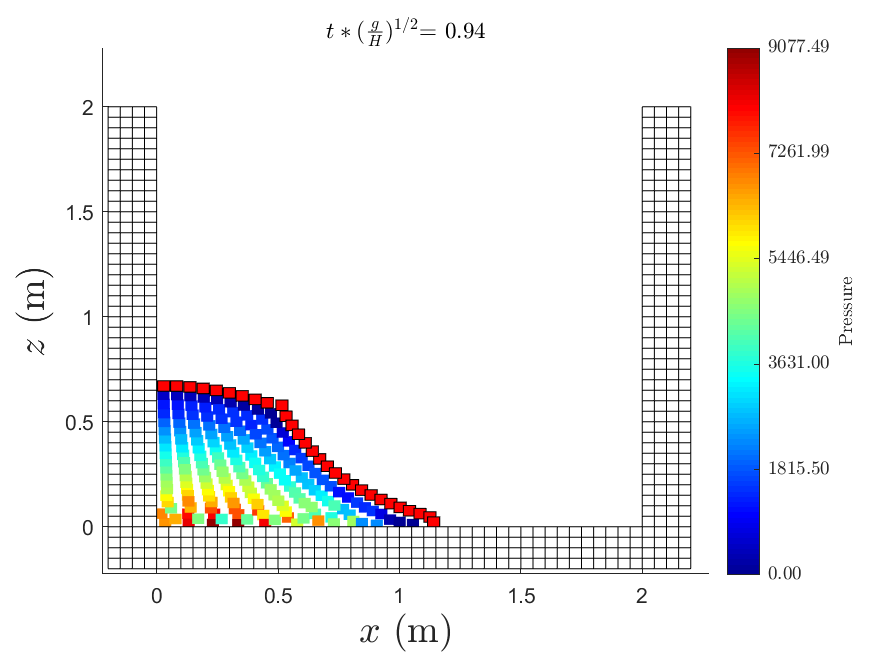
\includegraphics[width=1\linewidth]{img/sl/fig_000047}}
    \end{minipage}
    \vfill
    \begin{minipage}[h]{0.32\linewidth}
        \center{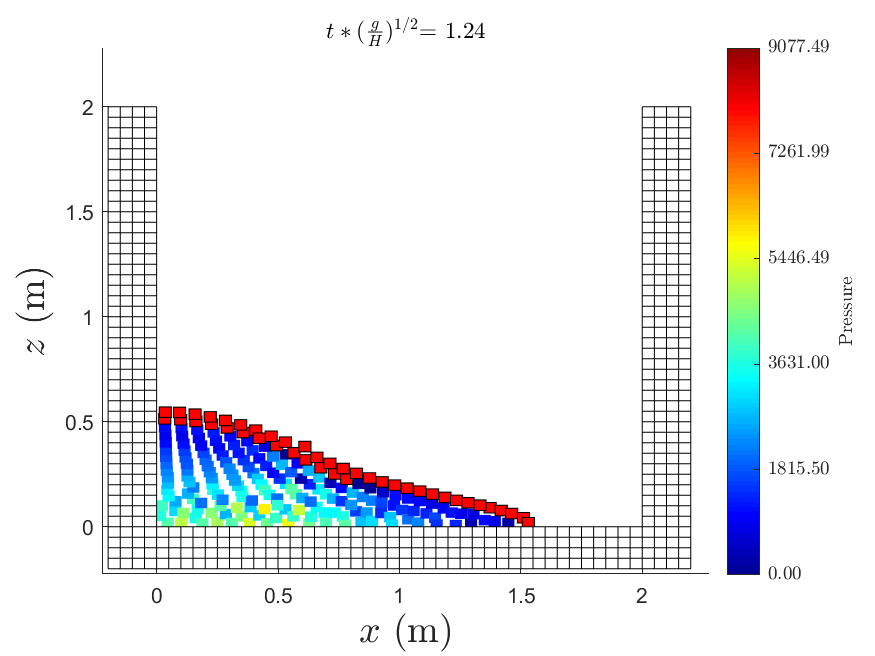
\includegraphics[width=1\linewidth]{img/sl/fig_000062}}
    \end{minipage}
    \hfill
    \begin{minipage}[h]{0.32\linewidth}
        \center{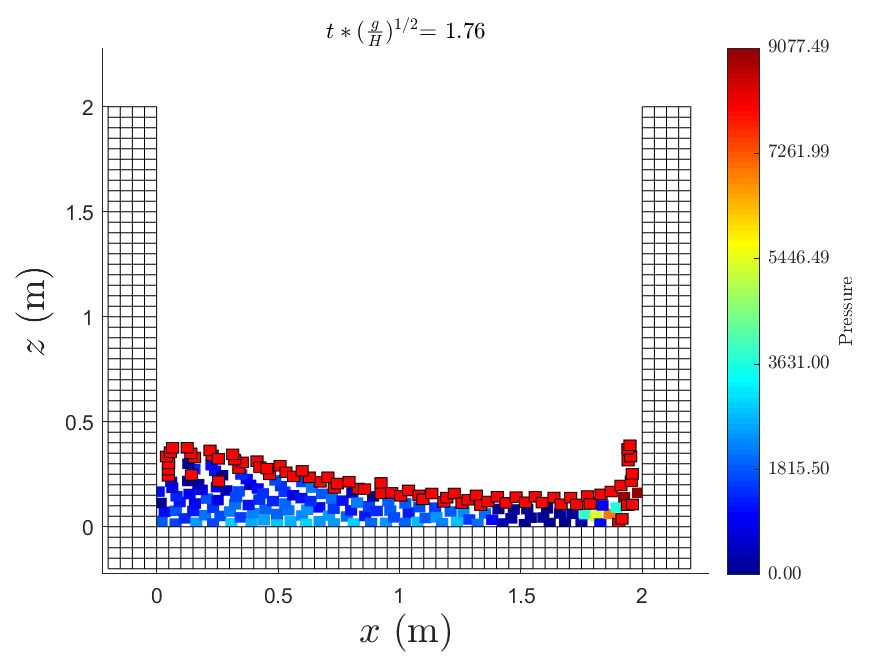
\includegraphics[width=1\linewidth]{img/sl/fig_000088}}
    \end{minipage}
    \hfill
    \begin{minipage}[h]{0.32\linewidth}
        \center{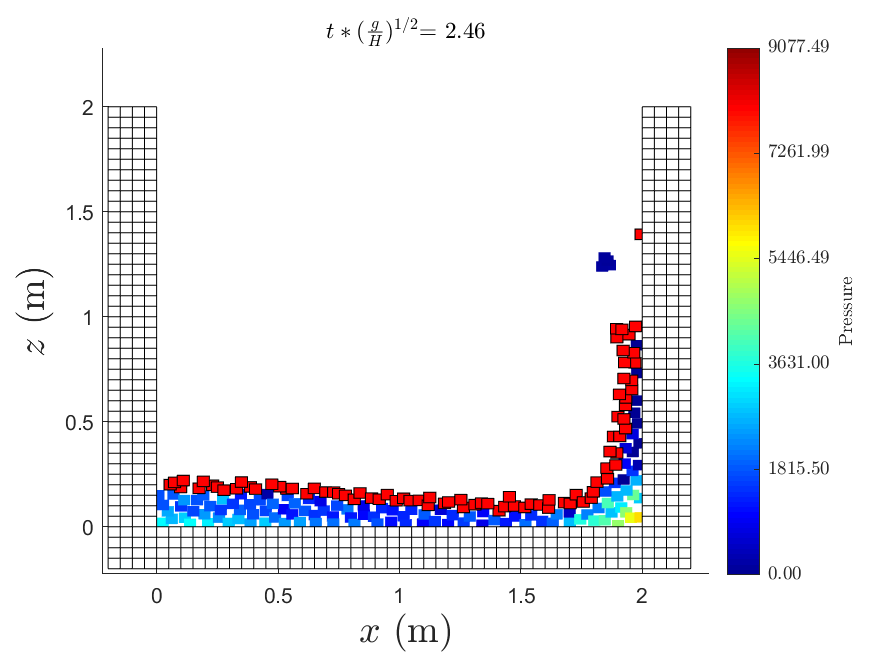
\includegraphics[width=1\linewidth]{img/sl/fig_000123}}
    \end{minipage}
    \vfill
    \begin{minipage}[h]{0.32\linewidth}
        \center{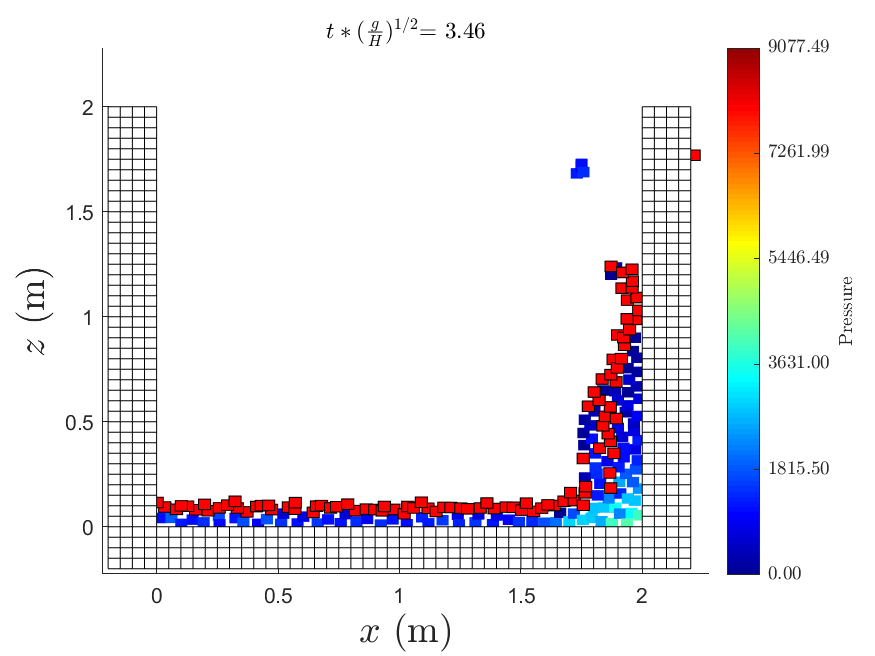
\includegraphics[width=1\linewidth]{img/sl/fig_000173}}
    \end{minipage}
    \hfill
    \begin{minipage}[h]{0.32\linewidth}
        \center{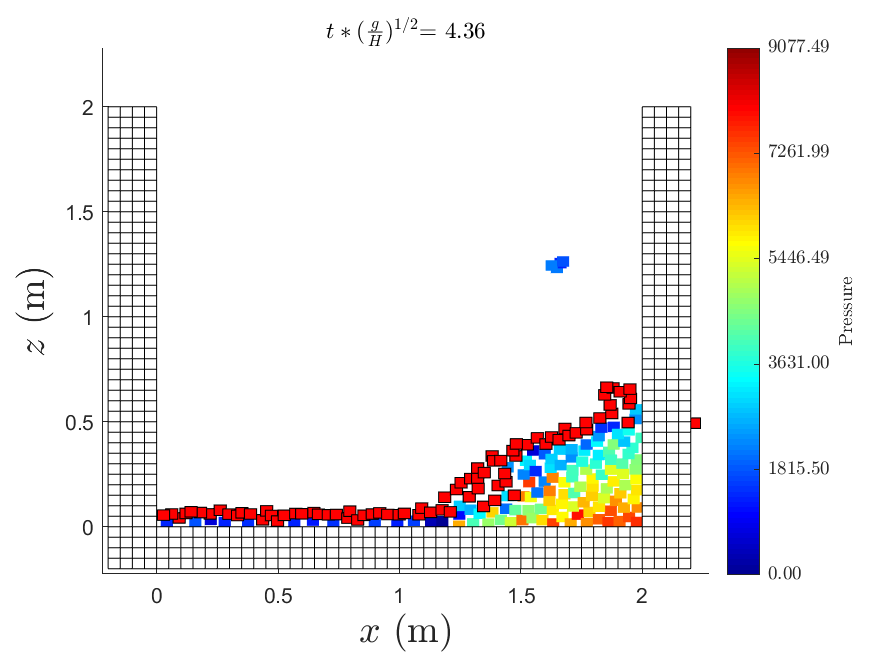
\includegraphics[width=1\linewidth]{img/sl/fig_000218}}
    \end{minipage}
    \hfill
    \begin{minipage}[h]{0.32\linewidth}
        \center{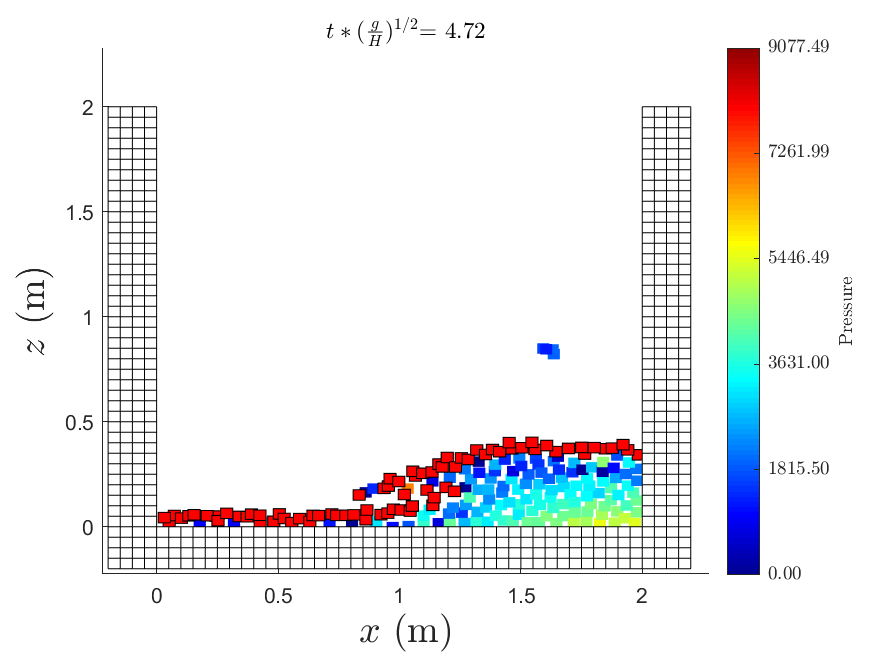
\includegraphics[width=1\linewidth]{img/sl/fig_000236}}
    \end{minipage}
    \caption{La démonstration de la surface libre pour les itérations différentes}
    % \label{ris:correlationsignals}
\end{figure}
    
Comme on voit l'algorithme fonctionne très bien sauf des certaines itérations. "La pénétration" des éléments de la surface libre puisse être liée avec l'inexactitude des calculs numériques et avec le petite nombre des particules. Cette méthode est suffisant pour approximer la surface libre. 
\end{document}